\documentclass[../BTOF_summary.tex]{subfiles}
 
\begin{document}
\section{Capabilities}

The content of this section is mainly based on work done by Dominik Steinschaden.
For a closer look at the exact methodology behind these concepts and further understanding of the limitations of these processes, the reader is advised to reference The \btof\ TDR (2017) and the dissertation \emph{"Optimization Studies and Performance Simulations for the Time-of-Flight System of PANDA"} (2018)¸ by D. Steinschaden\footnote{\url{https://panda.gsi.de/system/files/user_uploads/dominik.steinschaden/TH-PHD-2018-002.pdf}}.

The presented capabilities are all based on performance simulations using PandaRoot. The timing based analysis of this detectors data combined with momentum and track information from other detectors allows the \btofD\ to contribute two main features; event building and particle identification.

\subsection{Event Building}

Since \panda\ will not be equipped with a start time detector, the first challenge will be to group relevant hits into single events. This will have to be done before any further analysis of the data stream is possible. For this it is both important to capture all relevant hits and exclude all hits from other events.

For this step the time resolution of the respective detector is the qualifying factor. With average event rates in the high luminosity mode of up to \SI{20}{MHz} or respectively at intervals of \SI{50}{ns} and individual events at even smaller intervals, an excellent time resolution is required to avoid overlap of relevant detector hits. \fig~\ref{fig:Event_overlap} illustrates the difference a time resolution of \SI{100}{ps} makes compared to a time resolution of \SI{2}{ns}, where hits of multiple events overlap and can not be disentangled.

\begin{figure}[htbp]
	\centering
	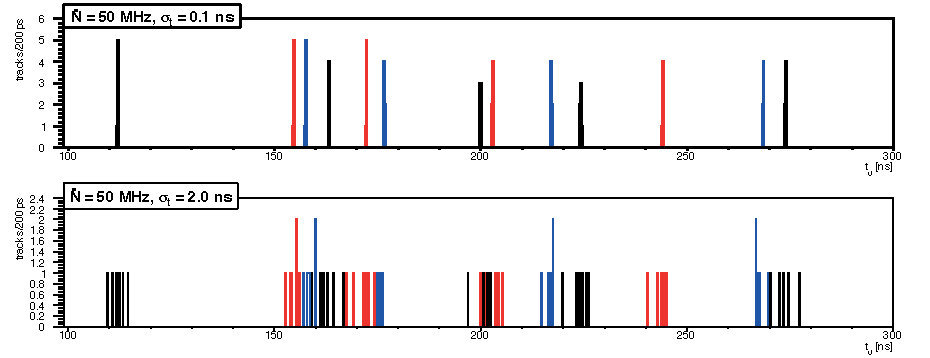
\includegraphics[width = .9\textwidth]{fig/Event_overlap.pdf}
	\caption{Simulation of the hit distribution for an average interaction rate of \SI{50}{MHz} and a detector resolution of \SI{0.1}{ns} and \SI{2}{ns} respectively.}
	\label{fig:Event_overlap}
\end{figure}


\subsection{Particle Identification and Event Time Determination}

Usually these two tasks are separated and handled by dedicated detectors.
After a start time is determined and a time stamp for a detector hit can be established, the time-of-flight of the respective particle can be calculated.
Combining this information with trajectory length and momentum information provided by the tracking detectors a velocity and hence a mass and particle identity can be determined.
Since \panda\ however has no start time detector, the event time has to be implicitly determined, by combining information of multiple detector hits and various detectors.
The technique used for this is called \emph{Relative Time-of-Flight} and delivers the event time and the respective particle identities of all involved hits simultaneously.

If a hit is registered in the \btofD\ it can not be a very short lived particle due to its radial distance of about \SI{50}{cm} to the interaction point.
This leaves a limited selection of possible particle candidates.
For grouped hits belonging to a single event the procedure is illustrated in \fig ~\ref{fig:relToF}.
Using tracking and momentum information from other detectors, the corresponding interaction time ($t_0$) in the interaction point of every \btof\ hit, can be calculated.
Iterating through all possible mass assumptions produces a distribution of possible $t_0$.
 
\begin{figure}
	\centering
	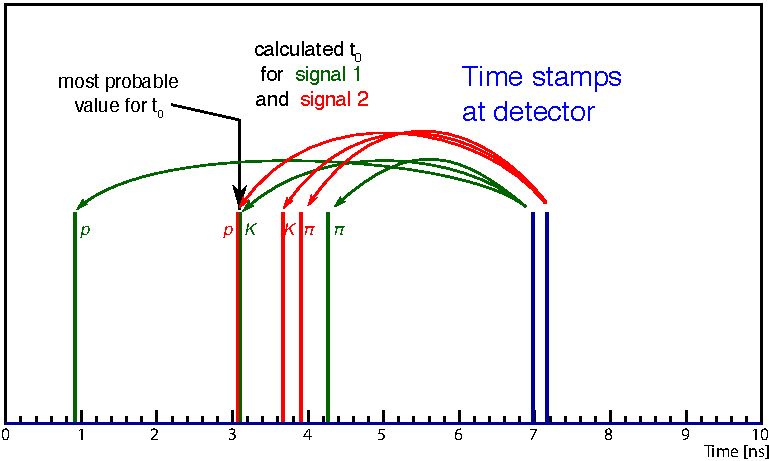
\includegraphics[width=.9\textwidth]{fig/relTof_basic.pdf}
	\caption{The relative time of flight method works by taking multiple mass assumptions of all involved detector hits here marked with blue lines on the time axis. Different particles show differences in their time-of-flight for the same momentum and trajectory due to differences in their mass and hence velocity. For these assumptions the respective interaction or creation time ($t_0$) is calculated and shown color coded; green for the first and red for the second hit. Where interaction times align we assume to have found $t_0$.}
	\label{fig:relToF}
\end{figure}

Since all hits belong to the same event a cluster of possible $t_0$ values with one candidate from every hit, should emerge.
Taking the mean of these candidate times in the cluster provides us with an estimation of the interaction time, as well as assigning the most likely particle mass to all involved particles.
Thereby identifying the particle species.

\end{document}